\documentclass[letterpaper,twocolumn,10pt]{article}
\usepackage{usenix2019_v3}

\usepackage{microtype}
\usepackage[leqno]{amsmath}
\allowdisplaybreaks
\usepackage{amssymb}
\usepackage{mathtools}
\usepackage{amsthm}
\usepackage{graphicx}
\usepackage{enumerate}
\usepackage{stmaryrd}
\usepackage{setspace}
\usepackage{tikz}
\usepackage{cleveref}
\usetikzlibrary{matrix}
%\usepackage{hyperref}
%you can add more packages using the same code above

\usepackage[color=yellow,textsize=scriptsize]{todonotes}
\setlength{\marginparwidth}{1.5cm}

%------------------

%\setlength{\topmargin}{0.0in}
%\setlength{\textheight}{10in}
%\setlength{\oddsidemargin}{0.0in}
%\setlength{\evensidemargin}{0.0in}
%\setlength{\textwidth}{6.5in}

%-------------------
\newtheorem{theorem}{Theorem}[section]
\newtheorem{proposition}[theorem]{Proposition}
\newtheorem{lemma}[theorem]{Lemma}
\newtheorem{corollary}[theorem]{Corollary}
\newtheorem{conjecture}[theorem]{Conjecture}

\theoremstyle{definition}
\newtheorem{definition}[theorem]{Definition}
\newtheorem{assumption}[theorem]{Assumption}
\newtheorem*{example}{Example}

%------------------

%Everything before begin document is called the pre-amble and sets out how the document will look
%It is recommended you don't touch the pre-amble until you are familiar with LateX

\newcommand{\defeq}{\triangleq}
\newcommand{\conj}{\mathrel\land}
\newcommand{\disj}{\mathrel\lor}

\newcommand{\awa}[2]{\mathrlap{#2}\hphantom{#1}} % as wide as

\renewcommand{\i}[1]{\ensuremath{\mathit{#1}}}

\newcommand{\Spec}{\ensuremath{\mathbb S}}
\newcommand{\Prog}{\ensuremath{\mathbb P}}
\newcommand{\ProgInv}{\ensuremath{\mathbb P^\dagger}}

\newcommand{\actw}{\mathsf w}
\newcommand{\actwc}{\mathsf w^\mathsf{c}}
\newcommand{\actf}{\mathsf f}
\newcommand{\actr}{\mathsf r}
\newcommand{\actfc}{\mathsf{f^c}}
\newcommand{\actrc}{\mathsf{r^c}}

\newcommand{\ttIn}[2]{\xrightarrow{#1}_{#2}}
\newcommand{\ttsIn}[2]{\xrightarrow{#1}^{\raisebox{-3pt}{\scriptsize\ensuremath{*}}}_{#2}}
\newcommand{\ttP}[1]{\ttIn{#1}{\Prog}}
\newcommand{\ttsP}[1]{\ttsIn{#1}{\Prog}}
\newcommand{\ttS}[1]{\ttIn{#1}{\Spec}}
\newcommand{\ttsS}[1]{\ttsIn{#1}{\Spec}}


\begin{document}

\title{Crash-Determinacy in Agda}
%\author{Lin Tzu Chi}
%\date{}
\maketitle

\begin{abstract}
We have proved crash-determininacy in Agda, assuming that some essential properties have been verified by an SMT solver.
\end{abstract}

%The following code is not run because of the percentage sign, but you might find it useful for future work
% \tableofcontents

\section{Overall Structure}

Recall that, to simplify the proof of crash-determinacy, we introduce an abstract (and simpler) transition system~\Spec\ that acts as a specification of the actual program transition system~\Prog.
Crash-determinacy will be established on~\Spec\ instead, and by making \Spec\ simulate~\Prog\ (a notion which we will define below), every well-formed fragment in~\Prog\ will correspond to one in~\Spec\ and be crash-deterministic.%
\todo{define crash-determinacy on fragments, and then on transition systems}\
The overall strategy for carrying out the proof is to use an SMT solver wherever possible, and verify the rest with a proof assistant, in this case Agda.
More specifically, the solver establishes the preservation of invariants in~\Prog\ and the simulation of~\Prog\ by~\Spec, and then with Agda we prove that \Spec\ is crash-deterministic, and that crash-determinacy of~\Spec\ does lead to crash-determinacy of~\Prog\ due to the simulation.

Below we will present the part of the proof formalized with Agda.
The Agda proof%
\todo{change to ``The majority of the Agda proof'' if eventually we need to prove stuff about the exact definitions of \i{AR}, \i{RI}, etc}\
does not depend on the detail of~\Prog, the invariants on program states, and the simulation of~\Prog\ by~\Spec, and these will be formulated as assumptions in \cref{sec:Prog}, where some notations will also be defined.
We will then define \Spec\ and prove its crash-determinacy in \cref{sec:Spec}.
Next we will formally define the simulation relation between \Prog~and~\Spec, but instead of considering the entire~\Prog, it suffices to focus on a sub-system~\ProgInv\ of~\Prog\ which consists of only the states satisfying the invariants and the transitions ``respecting'' the invariants; in \cref{sec:ProgInv} we will define~\ProgInv\ and prove some of its properties.
The simulation relation between \ProgInv~and~\Spec, to be defined in \cref{sec:sim}, will be easier to handle (compared to the one between \Prog~and~\Spec), and crash-determinacy of \ProgInv\ is the same as that of \Prog\ since the property is only about well-formed fragments,%
\todo{should probably be defined to start from initial states}\
which can be shown (in \cref{sec:ProgInv}) to be included in~\ProgInv.
The proof of crash-determinacy of~\ProgInv%
\todo{or a generalisation (requiring the starting state to be in a simulation)?}\
(and~\Prog) will then be presented in \cref{sec:proof}.

\section{The Program Transition System~\Prog}
\label{sec:Prog}

We assume that three sets are given,  
$$\i{Addr},\ \i{Data},\ \text{and}\ \i{ProgState}$$
where $\i{Addr}$ is the set of memory addresses, $\i{Data}$ the set of values of memory cells, $\i{ProgState}$ the set of all possible program states.
The exact definitions of these sets are irrelevant to the Agda proof and omitted.
We will need to read the memory cells in a program state, which is done by the function
$$ read : \i{ProgState} \to (\i{Addr} \to \i{Data}) $$
which returns the mapping from memory cell addresses to their values in a program state.

The (labelled) transition system~\Prog\ uses \i{ProgState} as its states, and its actions (labels) are defined by%
\todo{need to explain the meaning of the actions?}
\begin{align*}
%\noalign{\center{\small{State of Prog, we don't have to know the details.}}}
	\i{Action} \defeq{} &\{\, \actw_{\i{addr}, \i{data}} \mid \i{addr} \in \i{Addr}, \i{data} \in \i{Data} \,\} \\
	\cup \ &\{\, \actwc_{\i{addr}, \i{data}} \mid \i{addr} \in \i{Addr}, \i{data} \in \i{Data} \,\}\\
	\cup \ &\{ \actf, \actr, \actfc, \actrc \}
\end{align*}
Most of the time the pair of address and data in a $\actw$ or $\actwc$ action is not important, in which case we will omit the subscript.
The ternary (single-step) transition relation of~\Prog\ is
$${\ttP{}} \subseteq \i{ProgState} \times \i{Action} \times \i{ProgState}$$
Its exact definition is, again, irrelevant and omitted.
We write
$$s \ttP{a} s'$$
when state~$s$ transits to~$s'$ through action~$a$ in~\Prog.

Recall that there are two types of invariants on the states, the representation invariant \i{RI} and the crash invariant \i{CI}, which are preserved or transformed by the transitions; these properties are proved by an SMT solver, and are made assumptions in this proof.
\begin{assumption}[per-operation correctness]
For all $s$, $s' \in \i{ProgState}$, the following are assumed:
\begin{align*}
s \ttP{\awa{\actw}{\actw }} s' \conj \i{RI}(s) &\implies \i{RI}(s')\\
s \ttP{\awa{\actw}{\actf }} s' \conj \i{RI}(s) &\implies \i{RI}(s')\\
s \ttP{\awa{\actw}{\actwc}} s' \conj \i{RI}(s) &\implies \i{CI}(s')\\
s \ttP{\awa{\actw}{\actfc}} s' \conj \i{RI}(s) &\implies \i{CI}(s')\\
s \ttP{\awa{\actw}{\actr }} s' \conj \i{CI}(s) &\implies \i{RI}(s')\\
s \ttP{\awa{\actw}{\actrc}} s' \conj \i{CI}(s) &\implies \i{CI}(s')
\end{align*}
\end{assumption}

Below we will often need to talk about sequences of transitions in \Prog\ and other transition systems, and a general definition will be helpful.
\begin{definition}[fragments]
Let $T = (S, \Lambda, \ttIn{}{})$~be a labelled transition system.
A \emph{fragment} in~$T$ is a sequence of transitions
$$ s_0 \ttIn{a_1}{} s_1 \ttIn{a_2}{} \cdots \ttIn{a_n}{} s_n $$
where $s_i \in S$ and $a_j \in \Lambda$ for all $i$~and~$j$.
We sometimes omit the intermediate states and write
$$ s_0 \ttsIn{a_1a_2\ldots a_n}{} s_n $$
Note that a fragment may contain no transitions, in which case the starting and ending states are the same: 
$$ s_0 \ttsIn{\vphantom{a_n}}{} s_0 $$
\end{definition}


\section{The Specification Transition System~\Spec}
\label{sec:Spec}

For the transition system~\Spec, its states are those in the set
$$ \i{SpecState} \defeq (\i{Addr} \to \i{Data}) \times (\i{Addr} \to \i{Data}) $$
which contains pairs of mappings from \i{Addr} to \i{Data}; these two mappings represent the volatile and stable parts of a state in the specification respectively.%
\todo{define \i{volatile} and \i{stable}}\
The actions of~\Spec\ are the same as those of~\Prog.
The transition relation
$$ {\ttS{}} \subseteq \i{SpecState} \times \i{Action} \times \i{SpecState} $$
is defined by%
\todo{revise}
\begin{align*}
	\llbracket \mathsf w_{addr, data} \rrbracket ={}& \{\, (s, s') \in SpecState \times SpecState\\ &\mid \i{volatile(s)[addr \mapsto data]} \equiv \i{volatile(s')}
	\land stable(s) \equiv stable(s') \,\} \\
	\llbracket \mathsf f \rrbracket ={}& \{\, (s, s') \in SpecState \times SpecState\\ & \mid \i{volatile(s)} \equiv \i{volatile(s')} \land \i{volatile(s)} \equiv \i{stable(s')}\,\} \,\} \\
	\llbracket \mathsf r \rrbracket ={}& \{\, (s, s') \in SpecState \times SpecState\\ & \mid\i{stable(s)} \equiv \i{volatile(s')} \land \i{stable(s)} \equiv \i{stable(s')} \,\} \\
	\llbracket \mathsf {w^c} \rrbracket ={}& \{\, (s, s') \in SpecState \times SpecState\\ & \mid\i{stable(s)} \equiv \i{stable(s')} \,\} \\
	\llbracket \mathsf {f^c} \rrbracket ={}& \{\, (s, s') \in SpecState \times SpecState\\ & \mid\i{volatile(s)} \equiv \i{stable(s')} \lor \i{stable(s)} \equiv \i{stable(s')} \,\} \\
	\llbracket \mathsf {r^c} \rrbracket ={}& \{\, (s, s') \in SpecState \times SpecState\\ & \mid\i{stable(s)} \equiv \i{stable(s')} \,\}
\end{align*}

\section{The Sub-System~\ProgInv\ with Invariants}
\label{sec:ProgInv}

\section{Simulation of~\ProgInv\ by~\Spec}
\label{sec:sim}

\begin{align*}
\i{ProgState^{\dagger}} ={} &\{\, \i{rs} \in \i{ProgState} \mid \i{RI(rs) \lor CI(rs)} \,\}
\end{align*}


\section{Proof of Crash-Determinacy}
\label{sec:proof}

\section{Datatypes}


$ProgState^\dagger$ is a subset of $ProgState$ we care \---- states that satisfies either Representation Invariance or Crash Invariance. $Action$ is the set of all possible actions, and $\i{Fragment}$ is of all possible sequences of actions. ($^*$ is Kleene star)

And we need functions to represent actions of reading from states:
\begin{align*}
	volatile &: \i{SpecState} \to (\i{Addr} \to \i{Data})\\
	stable &: \i{SpecState} \to (\i{Addr} \to \i{Data})
\end{align*}

\newpage


transitions on $\i{SpecState}$ and $\i{ProgState^\dagger}$ are defined as families of relations $\{ \llbracket a \rrbracket \}_\i{a \in Action}$ and $\{ \llbracket a \rrbracket^\dagger \}_\i{a \in Action}$, with each relation defined as follows:
\begin{align*}
	\llbracket \mathsf w_{addr, data} \rrbracket^\dagger ={}& \{\, (s, s') \in ProgState^\dagger \times ProgState^\dagger\\ &\mid s \llbracket \mathsf w \rrbracket^P s' \land \i{RI(s)} \land \i{RI(s')} \,\} \\
	\llbracket \mathsf f \rrbracket^\dagger ={}& \{\, (s, s') \in ProgState^\dagger \times ProgState^\dagger\\ &\mid s \llbracket \mathsf f \rrbracket^P s' \land \i{RI(s)} \land \i{RI(s')} \,\} \\
	\llbracket \mathsf r \rrbracket^\dagger ={}& \{\, (s, s') \in ProgState^\dagger \times ProgState^\dagger\\ &\mid s \llbracket \mathsf r \rrbracket^P s' \land \i{CI(s)} \land \i{RI(s')} \,\} \\
	\llbracket \mathsf {w^c} \rrbracket^\dagger ={}& \{\, (s, s') \in ProgState^\dagger \times ProgState^\dagger\\ &\mid s \llbracket \mathsf {w^c} \rrbracket^P s' \land \i{RI(s)} \land \i{CI(s')} \,\} \\
	\llbracket \mathsf {f^c} \rrbracket^\dagger ={}& \{\, (s, s') \in ProgState^\dagger \times ProgState^\dagger\\ &\mid s \llbracket \mathsf {f^c} \rrbracket^P s' \land \i{RI(s)} \land \i{CI(s')} \,\} \\
	\llbracket \mathsf {r^c} \rrbracket^\dagger ={}& \{\, (s, s') \in ProgState^\dagger \times ProgState^\dagger\\ &\mid s \llbracket \mathsf {r^c} \rrbracket^P s' \land \i{CI(s)} \land \i{CI(s')} \,\} 
\end{align*}

For each of $\i{SpecState}$, $\i{ProgState}$ and $\i{ProgState^\dagger}$, a multi-step transition is defined as a transitive closure of its single-step transition:
\begin{align*}
	\bigcup_{i=1}^\infty\left(\bigcup_{a \in Action} \llbracket a \rrbracket \right)^i \quad
	\bigcup_{i=1}^\infty\left(\bigcup_{a \in Action} \llbracket a \rrbracket^P \right)^i \quad
	\bigcup_{i=1}^\infty\left(\bigcup_{a \in Action} \llbracket a \rrbracket^\dagger \right)^i \\
\end{align*}

Notice that any relation $r^i$ in closure $\bigcup_{i=1}^\infty\left(\bigcup_{a \in Action} \llbracket a \rrbracket \right)^i$ that belongs to $i$-th power of $\bigcup_{a \in Action} \llbracket a \rrbracket$ is a composition of a single-step relation $\llbracket a_1 \rrbracket$ and a relation $r^{i-1}$ which belongs to (${i-1}$)-th power of $\bigcup_{a \in Action} \llbracket a \rrbracket$:
$$r^i = \llbracket a_1 \rrbracket \circ r^{i-1}$$

By recursive decomposition, we can find a sequence of actions $a_i, a_{i-1}, a_{i-2} \dots a_1$, which maps to an unique fragment $\i{ef} = a_i \cdot a_{i-1} \cdot a_{i-2} \dots a_1$, thus each transitive closure of single-step transitions can be replaced with a family of relations indexed by $\i {Fragment}$:
\begin{align*}
	\{ \llbracket \i{ef} \rrbracket^* \}_\i{ef \in Fragment} &= 
	\bigcup_{i=1}^\infty\left(\bigcup_{a \in Action} \llbracket a \rrbracket \right)^i \quad\\
	\{ \llbracket \i{ef} \rrbracket^{P*} \}_\i{ef \in Fragment} &= 
	\bigcup_{i=1}^\infty\left(\bigcup_{a \in Action} \llbracket a \rrbracket^P \right)^i \quad\\
	\{ \llbracket \i{ef} \rrbracket^{\dagger*} \}_\i{ef \in Fragment} &= 
	\bigcup_{i=1}^\infty\left(\bigcup_{a \in Action} \llbracket a \rrbracket^\dagger \right)^i
\end{align*}

Important predicates and their meanings are given as follows:
\begin{align*}
	\i{Init^P(rs : ProgState)} &: \text{$\i{rs}$ is an initial state.}\\
	\i{RI(rs : ProgState)} &: \text{$\i{rs}$ satisfies Representation Invariance.} \\
	\i{CI(rs : ProgState)} &: \text{$\i{rs}$ satisfies Crash Invariance.} \\
	\i{AR(rs : ProgState, s : SpecState)} &: \text{$\i{rs}$ and $s$ satisfies Abstract Relation.} \\
	\i{CR(rs : ProgState, s : SpecState)} &: \text{$\i{rs}$ and $s$ satisfies Crash Relation.} \\
\end{align*}

Lemmas that are trivial or have been proved with theorem prover can be assumed here:
\begin{align*}
	%%\i{ExistsSpec} &: \forall t \in \i{State}, a \in \i{Action} \ldotp \exists t' \in \i{State} \ldotp t \llbracket a \rrbracket t'\\
	\tag{Observational Equivalence} & \forall \i{rs} \in \i{ProgState},s \in \i{SpecState} \ldotp \\
	& \qquad \i{RI(rs)} \land \i{AR(rs, s)} \implies \i{read(rs)} \equiv \i{volatile(t)} \\
	\tag{Initialization}\label{Initialization} &\forall \i{rs} \in \i{ProgState^\dagger} \ldotp\\
	&\qquad \i{Init(rs) \implies \exists s \in SpecState \ldotp RI(rs) \land AR(rs, s)}\\
	&\i{\forall s, s' \in ProgState^\dagger, t, t' \in SpecState,}\\
	&...	 \quad a \in \{w, f\} \ldotp \i{s \llbracket a \rrbracket^P s' \land t \llbracket a \rrbracket t' \land AR(s, t) \implies AR(s', t')}\\
	&...	 \quad a \in \{w^c, f^c\} \ldotp \i{s \llbracket a \rrbracket^P s' \land t \llbracket a \rrbracket t' \land AR(s, t) \implies CR(s', t')}\\
	&...	 \quad a \in \{r\} \ldotp \i{s \llbracket a \rrbracket^P s' \land t \llbracket a \rrbracket t' \land CR(s, t) \implies AR(s', t')}\\
	&...	 \quad a \in \{r^c\} \ldotp \i{s \llbracket a \rrbracket^P s' \land t \llbracket a \rrbracket t' \land CR(s, t) \implies CR(s', t')}\\
\end{align*}

We can now proceed to state and prove the lemmas and the theorem.
%\cref{Initialization}

\subsection{Lemmas}

\begin{lemma}\label{lemma-2-1}
\begin{multline*}
	\forall s, s', s'' \in \i{SpecState} \ldotp s \llbracket \i{(w \lor f)\ast} \cdot f \rrbracket^* s' \land s' \llbracket \i{w\ast} \cdot w^c \cdot \i{r^c\ast} \cdot r \rrbracket^* s'' \\
	  \implies \i{volatile(s')} \equiv \i{volatile(s'')}
\end{multline*}
\end{lemma}
\begin{proof}
	$s'$ is related from some $s \in \i{SpecState}$ by $\llbracket f \rrbracket$, so
		$$\i{volatile(s')} \equiv \i{volatile(s)} \equiv \i{stable(s')}$$
	since any state related by $\llbracket w \rrbracket$, $\llbracket w^c \rrbracket$ or $\llbracket r^c \rrbracket$ has its stable unchanged from the state it's related from, there is an intermediate state $s'_i$ such that
		$$s' \llbracket {w*} \cdot w^c \cdot {r^c *} \rrbracket^* s'_i \land s'_i \llbracket r \rrbracket s'' \land stable(s') \equiv stable(s'_i)$$
	finally, by $\llbracket r \rrbracket$ we know that $\i{stable(s'_i) \equiv volatile(s'')}$, thus we have
		$$\i{volatile(s') \equiv stable(s') \equiv stable(s'_i) \equiv volatile(s'')}$$
\end{proof}

\begin{lemma}\label{lemma-2-2}
\begin{multline*}
      \forall s, s', s'', s''' \in \i{SpecState} \ldotp \\
      s \llbracket \i{(w \lor f)\ast} \cdot f \rrbracket s' \land
	  s' \llbracket \i{w\ast} \rrbracket^{P*} s'' \land
	  s'' \llbracket f^c \cdot \i{r^c\ast} \cdot r \rrbracket^{P*} s'''\\ \implies \i{volatile(s')} \equiv \i{volatile(s''')} \lor \i{volatile(s'')} \equiv \i{volatile(s''')}
\end{multline*}
\end{lemma}
\begin{proof}
	We can find two intermediate state $s''_i$, $s''_j$ , such that $$s'' \llbracket f^c \rrbracket^P s''_i \land s''_i \llbracket r^c* \rrbracket^{P*} s''_j \land s''_j \llbracket r \rrbracket^P s'''$$
	then by doing a case analysis on $s'' \llbracket f^c \rrbracket s''_i$, we know that either $$\i{volatile(s'') \equiv stable(s''_i)}$$ or $$\i{stable(s'') \equiv stable(s''_i)}$$
	if $\i{volatile(s'') \equiv stable(s''_i)}$, by substituting $s'$ with $s''$ in
	\cref{lemma-2-1}, we can obtain $$\i{volatile(s'') \equiv volatile(s''')}$$
	if $\i{stable(s'') \equiv stable(s''_i)}$, the proof is exactly the same with \cref{lemma-2-1}, thus $$\i{volatile(s') \equiv volatile(s''')}$$
\end{proof}

\begin{lemma}\label{lemma-1}
	\begin{align*}
		&\i{SR(s, t)} = \i{AR(s, t)} \lor \i{CR(s, t)}\\
		&\forall s, s' \in \i{ProgState^\dagger}, t \in \i{SpecState}, \i{ef} \in \i{Fragment} \ldotp\\
		&\qquad \qquad \qquad s \llbracket \i{ef} \rrbracket^{P*} s'  \land \i{SR(s, t)} \implies \exists t' \ldotp t\llbracket \i{ef} \rrbracket^* t' \land \i{SR(s', t')} \\
	\end{align*}
\end{lemma}
\begin{proof}
	By $\i{ExistsSpec}$, there exists $t' \in SpecState$, such that $t \llbracket \i{ef} \rrbracket t'$, and by Per Operation Correctness, $s \llbracket \i{ef} \rrbracket^P s'$, $t \llbracket \i{ef} \rrbracket t'$ and $\i{AR(s, t)} \lor \i{CR(s, t)}$ implies either $\i{AR(s', t')}$ or $\i{CR(s', t')}$. \\
	The lemma can be sketched as follows
	\begin{figure} [h] \centering
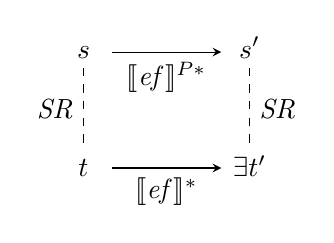
\begin{tikzpicture}
  \matrix (m) [matrix of math nodes,row sep=3em,column sep=4em,minimum width=2em]
  {
	  s & \vphantom{s}\smash{s'} \\
	 t & \vphantom{t}\smash{\exists t'} \\};
  \path[-stealth]
	(m-1-1) edge [dashed, -] node [left] {$\i{SR}$} (m-2-1)
			edge node [below] {$\llbracket \i{ef} \rrbracket^{P*}$} (m-1-2)
	(m-2-1) edge node [below] {$\llbracket \i{ef} \rrbracket^*$} (m-2-2)
	(m-1-2) edge [dashed, -] node [right] {$\i{SR}$} (m-2-2);
\end{tikzpicture}
	\end{figure}
\end{proof}

\section{Proof of theorem}

Similarly to lemmas, we separate the theorem into two parts, and alter it slightly to make it more consistent with what we have proved in Agda:

\begin{theorem}
\begin{multline*}
      \forall s, s', s'' \in \i{ProgState^\dagger} \ldotp\\\i{Init^P(s)} \land s \llbracket \i{(w \lor f)\ast} \cdot f \rrbracket^P s' \land s' \llbracket \i{w\ast} \cdot w^c \cdot \i{r^c\ast} \cdot r \rrbracket^P s'' \\ \implies \i{read(s')} \equiv \i{read(s'')}
\end{multline*}
\end{theorem}
\begin{proof}
	From $\i{initialisation}$ and repeatedly applying \cref{lemma-1} to the first relation, we have $\i{AR(s, t)}$ and $\i{AR(s', t')}$.
	The theorem can then be sketched as follows:
	\begin{figure} [h] \centering
		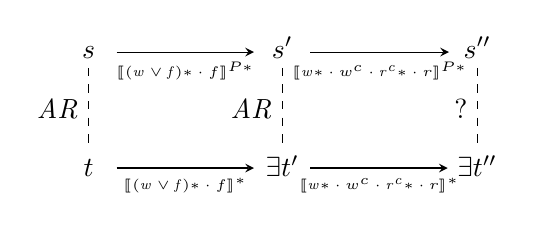
\begin{tikzpicture}
			\matrix (m) [matrix of math nodes, row sep=3em, column sep=5em, minimum width=2em]
			{ s & \vphantom{s}\smash{s'} & \vphantom{s}\smash{s''} \\
			  t & \vphantom{t}\smash{\exists t'} & \vphantom{t}\smash{\exists t''} \\};
			\path[-stealth]
			(m-1-1) edge [dashed, -] node [left] {$\i{AR}$} (m-2-1)
					edge node [below] {\tiny{$\llbracket \i{(w \lor f)*} \cdot f \rrbracket^{P*}$}} (m-1-2)
			(m-2-1) edge node [below] {\tiny{$\llbracket \i{(w \lor f)*} \cdot f \rrbracket^*$}} (m-2-2)
			(m-1-2) edge [dashed, -] node [left] {$\i{AR}$} (m-2-2)
					edge node [below] {\tiny{$\llbracket \i{w*} \cdot w^c \cdot \i{r^c*} \cdot r \rrbracket^{P*}$}} (m-1-3)
			(m-2-2) edge node [below] {\tiny{$\llbracket \i{w*} \cdot w^c \cdot \i{r^c*} \cdot r \rrbracket^*$}} (m-2-3)
			(m-1-3) edge [dashed, -] node [left] {?} (m-2-3);

		\end{tikzpicture}
	\end{figure}\\
	We can find some intermediate states $s'_1$, $s'_2$, $s'_3$, and by applying \cref{lemma-1} repeatedly to obtain
	\begin{figure} [h] \centering
		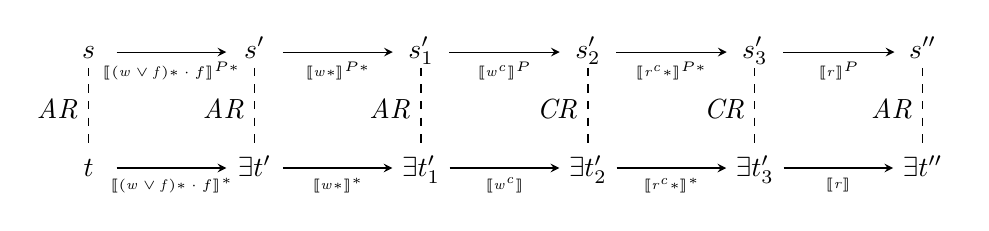
\begin{tikzpicture}
			\matrix (m) [matrix of math nodes, row sep=3em, column sep=4em, minimum width=2em]
			{ s & \vphantom{s}\smash{s'} & \vphantom{s}\smash{s'_1} & \vphantom{s}\smash{s'_2} & \vphantom{s}\smash{s'_3} & \vphantom{s}\smash{s''} \\
			  t & \vphantom{t}\smash{\exists t'} & \vphantom{t}\smash{\exists t'_1} & \vphantom{t}\smash{\exists t'_2} & \vphantom{t}\smash{\exists t'_3} & \vphantom{t}\smash{\exists t''} \\};
			\path[-stealth]
			(m-1-1) edge [dashed, -] node [left] {$\i{AR}$} (m-2-1)
					edge node [below] {\tiny{$\llbracket \i{(w \lor f)*} \cdot f \rrbracket^{P*}$}} (m-1-2)
			(m-2-1) edge node [below] {\tiny{$\llbracket \i{(w \lor f)*} \cdot f \rrbracket^*$}} (m-2-2)
			(m-1-2) edge [dashed, -] node [left] {$\i{AR}$} (m-2-2)
					edge node [below] {\tiny{$\llbracket \i{w*}  \rrbracket^{P*}$}} (m-1-3)
			(m-2-2) edge node [below] {\tiny{$\llbracket \i{w*} \rrbracket^*$}} (m-2-3)
			(m-1-3) edge [dashed, -] node [left] {$\i{AR}$} (m-2-3)
					edge node [below] {\tiny{$\llbracket \i{w^c}  \rrbracket^{P}$}} (m-1-4)
			(m-2-3) edge node [below] {\tiny{$\llbracket \i{w^c} \rrbracket$}} (m-2-4)
			(m-1-4) edge [dashed, -] node [left] {$\i{CR}$} (m-2-4)
					edge node [below] {\tiny{$\llbracket \i{r^c*}  \rrbracket^{P*}$}} (m-1-5)
			(m-2-4) edge node [below] {\tiny{$\llbracket \i{r^c*} \rrbracket^*$}} (m-2-5)
			(m-1-5) edge [dashed, -] node [left] {$\i{CR}$} (m-2-5)
					edge node [below] {\tiny{$\llbracket \i{r}  \rrbracket^{P}$}} (m-1-6)
			(m-2-5) edge node [below] {\tiny{$\llbracket \i{r} \rrbracket$}} (m-2-6)
			(m-1-6) edge [dashed, -] node [left] {$\i{AR}$} (m-2-6);

		\end{tikzpicture}
	\end{figure}\\
	thus complete the proof:
\begin{align*}
	\i{read(s)}   &\equiv \i{volatile(t)}   \tag{Observational Equivalence} \\
	& \qquad \quad \rotatebox{90}{$\equiv$} \tag{\cref{lemma-2-1}}\\
	\i{read(s'')} &\equiv \i{volatile(t'')} \tag{Observational Equivalence}
\end{align*} `
\end{proof}

\begin{theorem}
\begin{multline*}
      \forall s, s', s'', s''' \in \i{ProgState^\dagger} \ldotp\\\i{Init^P(s)} \land s \llbracket \i{(w \lor f)\ast} \cdot f \rrbracket^P s' \land
      s' \llbracket \i{w\ast} \rrbracket^P s'' \land
      s'' \llbracket f^c \cdot \i{r^c\ast} \cdot r \rrbracket^P s'''\\
      \implies \i{read(s')} \equiv \i{read(s''')} \lor \i{read(s'')} \equiv \i{read(s''')}
\end{multline*}
\end{theorem}


\end{document}
